\section{Beispiele f�r Zufallsvariablen und ihre Verteilungen}

Sei $(\Omega,\mathfrak{A},P)$ W-Raum und $X:\Omega\rightarrow\mathbb{R}$ reelle Zufallsvariable. 
$X$ hat dann eine Dichtefunktion (oder kurz "`Dichte"') $f(\geq 0)$, wenn gilt
\begin{equation}
	F(x) = P(X \leq x) = \int_{- \infty}^{+ \infty}{f(t) dt},\ -\infty < x < + \infty
\end{equation}

....

\subsection{Die Rechteck- oder Gleichverteilung}

$X$ hei�t gleichverteilt oder Rechteck-verteilt auf $[a,b]$. Die Schreibweise hierf�r sieht aus wie folgt
\[ X \sim \mathfrak{R}(a,b) \]

Soviel zu Rechteck- und Gleich-verteilung.

\subsection{Die Normalverteilung}

\begin{equation}
	f(t) = \frac{1}{\sqrt{2 \pi \sigma^2}} \cdot exp(- \frac{1}{2} \cdot \frac{(t - \mu )^2}{\sigma^2} ),\ - \infty < t < + \infty (\mu \in \mathbb{R}, \sigma^2 > 0)
\end{equation}
Die Dichte sieht aus wie folgt
\begin{equation}
	F(x) = P(X \leq x) = \int_{- \infty}^{+ \infty}{\frac{1}{\sqrt{2 \pi \sigma^2}} \cdot exp(- \frac{1}{2} \cdot \frac{(t - \mu )^2}{\sigma^2} )dt}
\end{equation}

F�r
\begin{itemize}
	\item $s := \frac{t-\mu}{\sigma}$
	\item $t = \mu + \sigma s$
	\item $dt = \sigma ds$
\end{itemize}
ist
(oben)

\begin{equation}
	\begin{split}
		% ref auf 48
		() &= \int_{- \infty}^{+ \infty}{\frac{1}{\sqrt{2 \pi }} \cdot exp(- \frac{1}{2} \cdot s^2 )dt} \\
			 &= \Phi \left( \frac{x-\mu}{\sigma} \right)\\
		\Phi(x) &= \frac{1}{\sqrt{2\pi}} \cdot \int_{- \infty}^{+ \infty}{exp(- \frac{1}{2} \cdot s^2 )dt},\ -\infty < x < +\infty
	\end{split}
\end{equation}

$X$ hei�t Normal-verteilt mit dem Parameter $\mu \in \mathbb{R}$ und $\sigma^2 > 0$.
Schreibweise:
\begin{equation}
	X \sim  N(\mu, \sigma^2)
\end{equation}

\subsubsection{Beispiele f�r Normalverteilungen}

\begin{itemize}
	\item 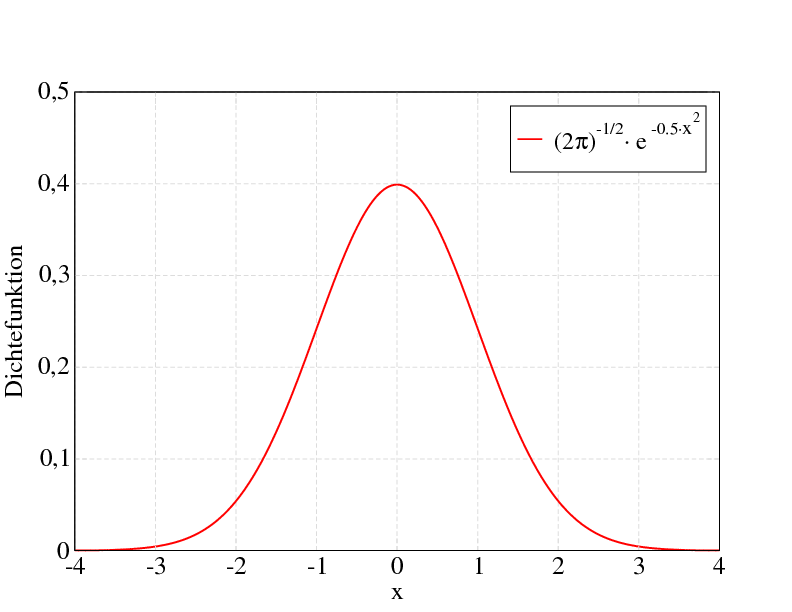
\includegraphics[scale=0.25]{Dichtefunktion_StNorm.png}\\
	Das \footnote{Quelle \href{http://de.wikipedia.org/wiki/Normalverteilung}{Wikipedia}} ist die so genannte Standard-Normal-Verteilung, auch bekannt als Gau\ss\ 'sche Glockenkurve
	\item 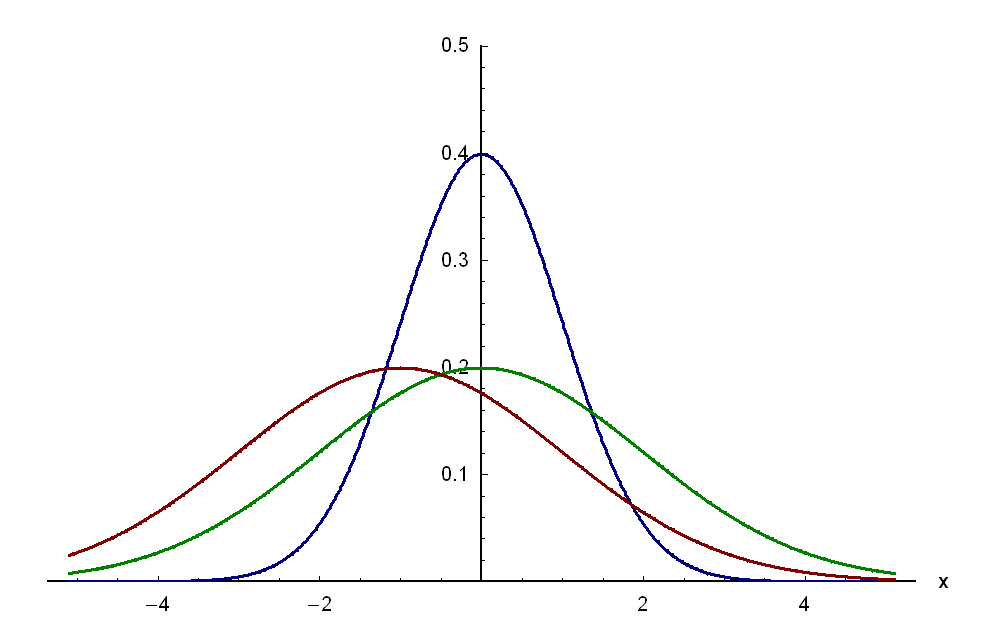
\includegraphics[scale=0.25]{Dichtefunktion_Norms.png}\\
	Zum Vergleich Dichtefunktionen der Normalverteilungen $N(0,1)$ (blau), $N(0,2)$ (gr�n) und $N(-1,2)$ (rot)
\end{itemize}

\subsection{Die Exponential-Verteilung}

\begin{equation}
	f(t) = \begin{cases}
		0 			&,\ t < 0\\
		\lambda \cdot exp(-\lambda t) &,\ t \geq 0
	\end{cases}
\end{equation}

Hierbei sei $\lambda > 0$.

Dann
\begin{equation}
	F(x) = P(X \leq x) = \begin{cases}
		0 			&,\ x < 0\\
		1 - exp(-\lambda t) &,\ x \geq 0
	\end{cases}
\end{equation}

$X$ hei�t Exponential-verteilt mit dem Parameter $\lambda > 0$.
Schreibweise:
\begin{equation}
	X \sim Exp(\lambda)
\end{equation}

% neuer abschnitt?

$X:\Omega \rightarrow \mathbb{R}^2$ sei ein 2-dimensoinaler Zufalsvektor, $X=(X_1,X_2)$.
$X$ habe die Dichte $f(\geq 0)$, d.h.
\begin{equation}
	\begin{split}
		P(X_1 \leq x_1, X_2 \leq x_2) &= \int_{-\infty}^{x_2}{\left( \int_{-\infty}^{x_1}{f(t_1,t_2) dt_2} \right)dt_1} \\
																	&= \int_{-\infty}^{x_1}{\left( \int_{-\infty}^{x_2}{f(t_1,t_2) dt_1} \right)dt_2}
	\end{split}
\end{equation}

Dann ist
\begin{equation}
	\begin{split}
		P(X_1 \leq x_1) &= \int_{-\infty}^{x_1}{\left( \int_{-\infty}^{+ \infty}{f(t_1,t_2) dt_2} \right)dt_1} \\
										&= \int_{- \infty}^{x_1}{f_{X_1}(t_1) dt_1}
	\end{split}
\end{equation}

Also ist 
\begin{equation}
	f_{X_1}(t_1) = \int_{- \infty}^{+ \infty}{f(t_1,t_2)dt_2},\ -\infty < t_1 < + \infty
\end{equation}
Dichte von $X_1$

Analog errechnet sich die Dichte von $X_2$

\part{Bedingte Wahrscheinlichkeiten}

\section{Bedingte Wahrscheinlichkeiten}

$(\Omega,\mathfrak{A},P)$ ist W-Raum.
Zun�chst $|\Omega| < \infty,\ \mathfrak{A} = \mathfrak{P}(\Omega),\ P(A)=\frac{|A|}{|\Omega|},\ A \subset \Omega,\ A\subset \Omega, B\subset\Omega, |B| \geq 1$.
Dann
\begin{equation}
	\frac{|A \cap B|}{|B|} = \frac{\frac{|A \cap B|}{|\Omega|}}{\frac{|B|}{|\Omega|}} = \frac{P(A \cap B)}{P(B)}
\end{equation}
"`Wahrscheinlichkeit f�r das Eintreten von A unter Bedingung, dass B eintritt"', lese als "`Wahrscheinlichket von A unter B"'

\subsection{Definition}

$(\Omega,\mathfrak{A},P)$ W-Raum (bel), $A,b \in \mathfrak{A}, P(B)>0$. Dann hei�t
\begin{equation}
	P(A|B) = \frac{P(A \cap B)}{P(B)}
\end{equation}
die bedingte Wahrscheinlichkeit von A unter B ("`A gegeben B"').

\subsection{Satz}

$(\Omega,\mathfrak{A},P)$ W-Raum, $\emptyset \neq I$ abz�hlbare Indexmenge.
Wir unterstellen $A_i \in \mathfrak{A}, i \in I$ seien paarweise disjunkt, $P(A_i) > 0$ f�r jede $i \in I$.
Dann halten wir fest
\begin{enumerate}
	\item F�r $A \in \mathfrak{A}$ mit der Eigenschaft $A \in \sum_{i \in I}{A_1}$ ist $P(A) = \sum_{i \in I}{P(A|A_i)P(A_i)}$ (bekannt als "`Satz von der totalen Wahrscheinlichkeit"')
	\item Sei $A \in \mathfrak{A}$ mit $P(A) > 0, i_0 \in I$. Dann
	\begin{equation}
		P(A_{i_0}|A) = \frac{P(A|A_{i_0})P(A_{i_0})}{\sum_{i \in I}{P(A|A_i)P(A_i)}}
	\end{equation}
	(bekannt als "`Formel von Bayes"')
	\item Sei $I = \{ 0,1,\ldots,n \},\ (n \in \mathbb{N} \text{fest})$. Dann gilt
	\begin{equation}
		P(A_0 \cap A_1 \cap \ldots \cap A_n) = P(A_0)P(A_1|A_0)P(A_2|A_0\cap A_1)\cdots P(A_n|A_0\cap \ldots \cap A_{n-1})
	\end{equation}
	(bekannt als "`Multiplikationsformel"')
\end{enumerate}

\subsection{Beweis}
\begin{enumerate}
	\item Aus \[A = \sum_{i\in I}{(A \cap A_i)} \] folge sofort
	\[ P(A) \sum_{i\in I}{P(A \cap A_i)} = \sum_{i\in I}{P(A|A_i)P(A_i)} \]
	\item folgt sofort aus 1.
	\item \begin{equation}
		\begin{split}
		& P(A_0)P(A_1|A_0)P(A_2|A_0\cap A_1)\cdots P(A_n|A_0\cap \ldots \cap A_{n-1}) \\
		=	& \cancel{P(A_0)}\cdot \frac{\cancel{P(A_1\cap A_0)}}{\cancel{P(A_0)}} \cdot \frac{P(A_0 \cap A_1 \cap A_2)}{\cancel{P(A_0 \cap A_1)}} \cdots \\
		= & P(A_0\cap A_1 \cap \ldots \cap A_n)
		\end{split}
  \end{equation}
\end{enumerate}

\subsection{Beispiel: Lostrommel}

Eine Lostrommel enth�lt $a$ Gewinnlose und $b$ Nieten, $A \geq 1, b \geq 2$. Es gibt $2$ Spielm�glichkeiten:
\begin{enumerate}
	\item Ein Los wird gezogen. Das gezogene Los ist ein Gewinnlos oder eine Niete. Das Spiel ist beendet.
	\item Ein Los wird gezogen und unbesehen weggeworfen. Daraufhin entfernt der Losverk�ufer eine Niete aus der Trommel. Ein weiteres Los wird gezogen. Dieses Los ist ein Gewinnlos oder eine Niete.
\end{enumerate}

Sei $A$ das Ereignis, dass bei der ersten Ziehung ein Gewinnlos gezogen wird.\\
Sei $B$ das Ereignis, dass bei der zweiten Ziehung ein Gewinnlos gezogen wird.

Dann ergibt sich bei diesen F�llen
\begin{enumerate}
	\item \begin{equation}
		P(A) = \frac{a}{a+b}
	\end{equation}
	\item \begin{equation}\begin{split}
		P(B) 	&= P(B|A)\cdot P(A) + P(B|A^c)P(A^c) \\
					&= \frac{a-1}{a+b-2}\cdot \frac{a}{a+b} + \frac{a}{a+b-2} \cdot \frac{b}{a+b} \\
					&= \frac{a}{a+b}\cdot\left(\underbrace{\frac{a+b-1}{a+b-2}}_{\geq 1} \right) > \frac{a}{a+b} > P(A)
		\end{split}
	\end{equation}
	Sei nun $a=1,\ b=2$. Dann folgt sofort
	\begin{equation*}
		\begin{split}
			P(A) &= \frac{1}{3}\\
			P(B) &= \frac{1}{3}\cdot 2 = \frac{2}{3}
		\end{split}
	\end{equation*}
\end{enumerate}

Sei $A,B \in \mathfrak{A}, P(B)>0$. Dann gilt offenbar
\begin{equation}
	P(A|B) = P(A) \iff P(A\cap B) = P(A)P(B)
\end{equation}

\section{Stochastische Unabh�ngigkeit von Ereignissen und Zufallsvariablen}

\subsection{Definition}

$(\Omega,\mathfrak{A},P)$ W-Raum, $A,B \in \mathfrak{A}$. $A,B$ hei�en (stochastisch) unabh�ngig, wenn \[ P(A \cap B) = P(A)P(B) \] gilt.

\subsection{Einsicht / Beweis}

\begin{equation}
	\begin{split}
		P(A \cap B^c)	&= P(A)-P(A \cap B) \\
									&= P(A) - P(A)P(B),\ \text{falls $A,B$ unabh�ngig} \\ % \Rightarrow A,B^c unabh�ngig
									& (1-P(B))P(A) \\
									&= P(A)P(B^c)
	\end{split}
\end{equation}

\subsection{Definition}
\begin{itemize}
	\item $\emptyset \neq I$ endliche Indexmenge, $A_i \in \mathfrak{A}, i \in I$ Ereignisse.\\
				$A_i$ hei�en (stochastisch) unabh�ngig, wenn f�r jede $\emptyset \neq J \subset I$ gilt
				\begin{equation}
					P\left( \bigcap_{j\in J}{A_j} \right) = \prod_{j \in J}{P(A_j)}
				\end{equation}
	\item $\emptyset \neq I$ beliebige Indexmenge, $A_i \in \mathfrak{A}, i \in I$ Ereignisse.\\
				$\mathfrak{A}_i, i \in I$ hei�en unabh�ngig, wenn f�r jede Teilmenge $\emptyset \neq J \subset I,\ J \text{endlich}$ die Ereignisse $A_j,j\in J$ unabh�ngig sind.
\end{itemize}

\subsubsection{Bemerkung}

$A_i \in \mathfrak{A}, i \in I$ seien Ereignisse. Dann gilt
\begin{equation}
	A_i, i\in I \text{ unabh�ngig } \iff B_i, i\in I \text{ unabh�ngig },\ B_i \in \{A_i, A_i^c\} \text{ beliebig}
\end{equation}

\subsection{Definition}

$(\Omega,\mathfrak{A},P)$ W-Raum, $\emptyset \neq I$ Indexmenge, $(R_i,\mathfrak{S})$ Messr�ume, $i \in I$,
$X_i:\Omega \rightarrow R_i$ Zufallsvariable, $i \in I$.\\
$X_i, i\in I$ hei�en (stochastisch) unabh�ngig, wenn f�r jede Wahl von $B_i \in \mathfrak{S}_i, i\in I$ die Ereignisse 
$A_i = X_i^{-1}(B_i), i \in I$ unabh�ngig sind.

\subsection{Spezialfall}
$I = \{1,\ldots,n\}$.

$X_i, i \in I$ sind unabh�ngig $\iff P(X_1 \in B_1, \ldots, X_n\in B_n) = P(X_1 \in B_1) \cdots P(X_n\in B_n), \forall B_i \in \mathfrak{S}_i, i \in I$

\begin{enumerate}
	\item $X_1,\ldots,X_n$ haben eine \textbf{diskrete Verteilung}. Dann
				\[ X_1,\ldots,X_n \iff P(X_1=x,\ldots,X_n=x_n) = P(X_1=x_1)\cdots P(X_n=x_n)\]
				f�r jede $x_i \in R_i, i \in I$
\end{enumerate}